This section describes the methodology that we followed during the development of our project, which is the waterfall model.

\subsection{Software Development Life Cycle}
For the development of our project, we chose to follow the waterfall model\cite{waterfall} of the software development life cycle as depicted in Figure \ref{fig:sdlc}. The reason for choosing this model was the lack of sufficient time duration for agile and iterative methods, as well as very low chances of changes of requirements in the process of development. 

\begin{figure}[h]
	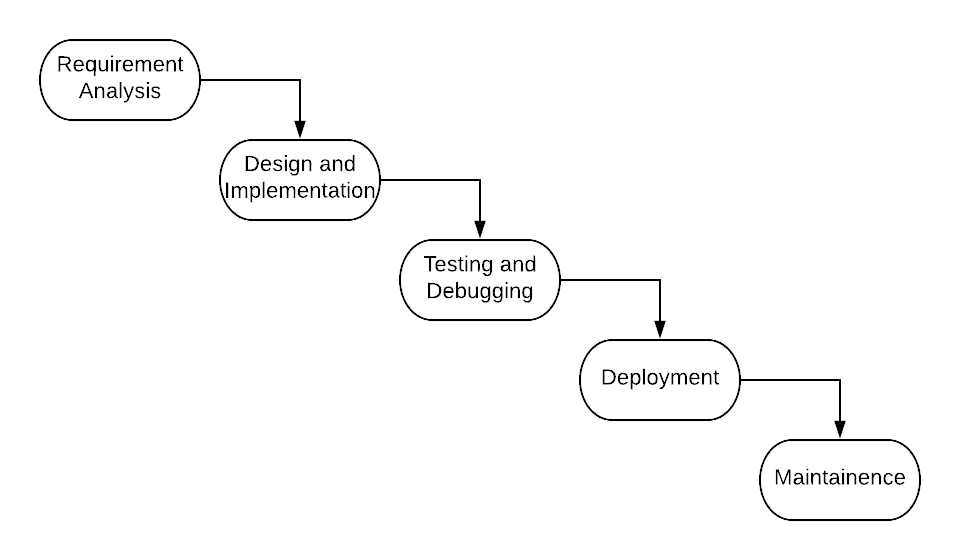
\includegraphics[width=\linewidth]{figures/sdlc.png}
	\centering
	\caption{ Software development life cycle}
	\label{fig:sdlc}
\end{figure}

For the development of our project, we adopted the waterfall model as our chosen software development life cycle. In this model, the project life cycle began with the collection and evaluation of requirements for the application. We then proceeded to the design and implementation phase, where we designed and built both the API services and client applications. By the end of this phase, we had a minimal viable product (MVP) constructed.

In the testing and debugging phases, the quality control methods were applied to both the API and application. However, there might have been slight modifications in the original waterfall model where the design and implementation were changed slightly after the testing phase if seen as reasonable.

\subsection{Technical Architecture}
The application was built upon the client-server web architecture, as illustratedin Figure.
\ref{fig:arch}. 
\begin{figure}[H]
    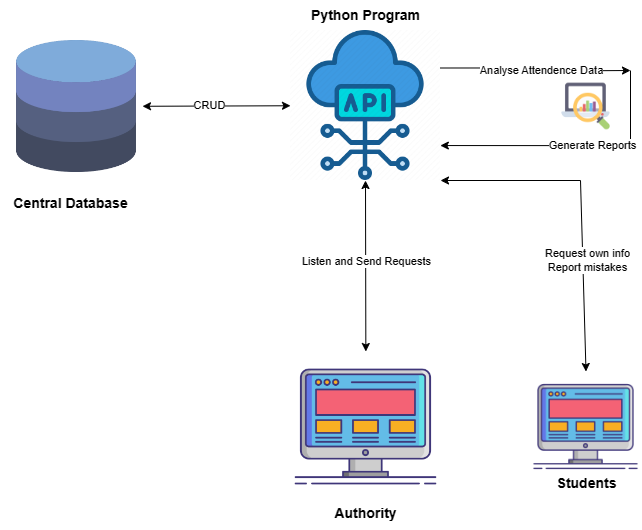
\includegraphics[width=\linewidth]{figures/architecture.png}
    \centering
    \caption{Architecture of the application}
    \label{fig:arch}
\end{figure}

The architecture consists of a database that handles data storage and management. Python is responsible for handling Create, Read, Update, and Delete (CRUD) operations on the database. It also provides WebSocket communication capabilities to the client application.\\

The client application allows students to access their personal attendance information securely. Only authorized personnel, such as administrators or instructors, can access the entire dataset via the client application using WebSocket communication.\\

Python program acts as the intermediary between the client application and is also responsible for generating reports based on the attendance data. This communication ensures seamless integration and efficient report generation.\\

\begin{figure}[H]
    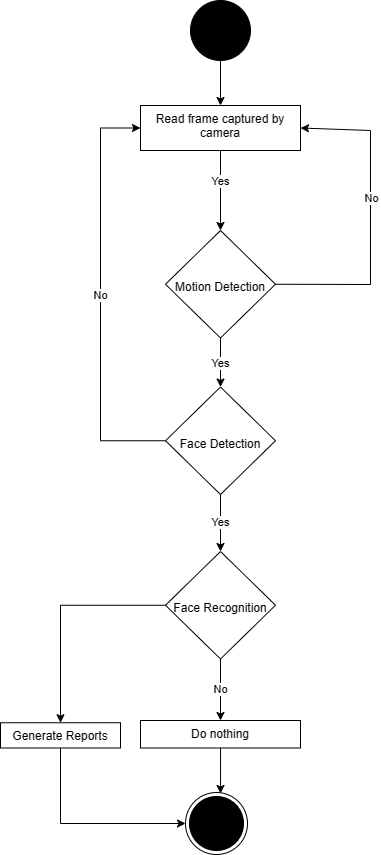
\includegraphics[width=0.6\linewidth]{figures/activity-diagram.png}
    \centering
    \caption{Activity Diagram\cite{yasmeensmart} of the application}
    \label{fig:activity}
\end{figure}

\begin{figure}[H]
    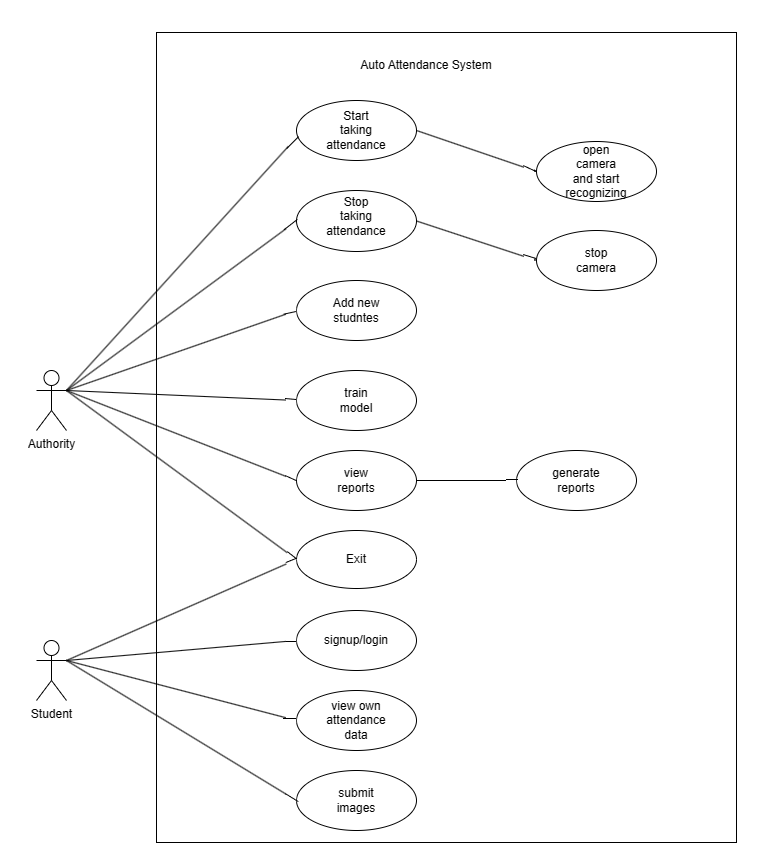
\includegraphics[width=\linewidth]{figures/use-case.png}
    \centering
    \caption{Use-case Diagram of the application}
    \label{fig:usecase}
\end{figure}

\subsection{Technologies}
Table \ref{table:tech} presents the major technologies that we used for the development and deployment of our application.

\renewcommand{\arraystretch}{1.5}
\begin{table}[H]
\centering
    \begin{tabular}{|l|l|}
        \hline
        \textbf{Subject}    & \textbf{Technology} \\ \hline
        Backend Database            &SQLite           \\ \hline
        Backend Service    & django, Python        \\ \hline
        API Communication & REST APIs and WebSocket \\ \hline
        Frontend(Client)  & Next.js(React), Typescript, TailwindCSS              \\ \hline
    \end{tabular}
    \caption{Technologies we used}
    \label{table:tech}
\end{table}

\subsection{Face detection algorithm}
For the development of our project, we utilized the OpenCV library in Python to train our model and perform face detection for attendance purposes. In this regard, we have two options for face detection: 
HOG(Histogram of Oriented Gradients) or CNN.\\


The HOG face detector offers faster processing speed, which aligns well with our limited resources and time constraints. It operates by dividing an image into small cells, computes each cell’s gradient orientation and magnitude, and then aggregates the gradient information into a histogram of oriented gradients. These histograms describe the image features and detect objects within an image. However, it may be less accurate when dealing with changes in the viewing angle or rotation of faces.\\

For more robust face detection, we can employ the CNN face detector. This approach requires more computational resources, resulting in slower processing times. Nonetheless, it offers higher accuracy and is more resilient to variations in face rotation and viewing angles.\\

Furthermore, if we have access to a GPU, we can leverage it to run the CNN face detector, enabling real-time face detection. Combining the CNN face detector with a GPU delivers the perfect combination of deep neural network accuracy and the efficiency of a less computationally demanding model.\\

We have used HOG(Histogram of Oriented Gradients) because of low resources and less time.\\



\begin{table}[H]
\centering
\resizebox{\textwidth}{!}{%
\begin{tabular}{|l|l|l|}
\hline
\textbf{Algorithm} & \textbf{HOG} & \textbf{CNN} \\
\hline
Approach & Histogram of Oriented Gradients (HOG) feature extraction & Convolutional Neural Network (CNN) \\
\hline
Training Complexity & Less computationally intensive & More computationally intensive \\
\hline
Speed & Faster & Slower \\
\hline
Accuracy & Less accurate, especially with changes in viewing angles & More accurate and robust to face rotation \\
\hline
Face Rotation Tolerance & Low & High \\
\hline
GPU Support & Limited (may not utilize GPU) & Utilizes GPU for improved performance \\
\hline
Model Size & Smaller & Larger \\
\hline
\end{tabular}%
}
\caption{Comparison of HOG and CNN algorithms for face detection.}
\label{table:algorithm_comparison}
\end{table}

\begin{figure}[H]
    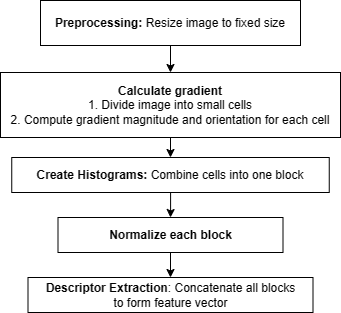
\includegraphics[width=0.8 \linewidth]{figures/hog-process.png}
    \centering
    \caption{Hog process of feature extraction}
    \label{fig:hog-process}
\end{figure}

\subsection{Flow of user in the platform}

\textbf{Admin}: 
\begin{itemize}

    \item Provides an admin panel where teachers, who are also admins, can add new student details.
    \item Admins then share these login details with students.
    \item Students use these credentials to log into the platform.
    \item Students can submit their images, which are processed using the HOG algorithm to create a pickle file containing facial details.
    \item Admins can take attendance using a camera.
    \item Real-time attendance logs are available in both text and video formats, which can be converted into reports.
\end{itemize}

\textbf{Student}: 
\begin{itemize}

    \item Students can log in using the credentials provided by their teachers.
    \item They have the option to request a password reset, which involves sending a reset link to their email.
    \item Clicking on the reset link verifies the provided tokens.
    \item Students can view their attendance in a calendar format.
    \item They can also track their attendance streak, which serves as a motivational factor.
\end{itemize}
